

Fuzz testing is a popular technique for automatic software vulnerability detection 
 \cite{Miller:Fuzz, 5010257, sutton2007fuzzing}.
 However, it suffers from the low efficiency bottleneck when being applied to real-world software 
 \cite{neystadt2008automated, godefroid2008automating, ganesh2009taint, cadar2011symbolic, rawat2017vuzzer, stephens2016driller},
  which often has complex input formats, e.g., Portable Document Format (PDF).
  Fuzz testing can only generate test cases that are discarded on the shallow surface of such software.
  %This is because modern software often has complex input formats, e.g., Portable Document Format (PDF), 
  %which determines that most of the test cases generated by fuzz testing will be discarded 
  %on the shallow surface of programs. 
  In order to improve the performance of traditional fuzz testing, 
  coverage-based fuzz testing collects all the test cases that contribute to the coverate into a seed file queue,
  and generates the test input from the seed files in each cycle of mutation using genetic methods
  \cite{rawat2017vuzzer, online:afl, stephens2016driller}.
  Although coverage-based testing is able to reach more paths than traditional fuzz testing, 
  due to the usage of genetic metods,
  it is nevertheless incapable of triggering bugs that are deeply nested in complex code areas,
  since it treats the software as a gray box.
  
% treating the software as a gray box determines it still cannot trigger the bugs 
%  that deeply nested in complex code areas.

% Coverage based fuzz testing improves the performance of traditional fuzz testing 
% by collecting all test cases that contribute to coverage into a seed file queue, 
% and all the test cases in this queue will be picked up as the template file for a new cycle of mutation.
% By utilizing such genetic method, 
% the fuzzer can quickly reach more paths and find more bugs than traditional fuzz testing. 


Another technique to improve the efficiency of fuzz testing is symbolic execution assisted hybrid testing \cite{yeh2015craxfuzz, majumdar2007hybrid, pak2012hybrid}.
 In such hybrid testing, symbolic execution is exploited to cover the corner cases that are difficult for classical fuzzers to cover by solving the corresponding path conditions.
 Meanwhile, symbolic execution can also benefit from the seed files in the queue from fuzzer 
 to quickly reach more wider code areas. 
 Driller, which is built on top of Angr symbolic execution engine \cite{Shoshitaishvili_firmalice-automatic} and AFL fuzzing engine \cite{online:afl}, 
 has attempted to leverage symbolic execution to solve the branches guarded 
 by complex path conditions to avoid the saturation of fuzzer \cite{stephens2016driller}. 
 And its performance in the CGC challenge \cite{online:CGC} demonstrates the potential of this hybrid testing approach.

{\color{blue}{1: explain that in hybrid testing, software is not taken as a gray box.
 2: explain what CGC is, give the full name. 3: are there some other hybrid testing? 
 why do you say symbolic execution assisted? 4: say that hybrid testing is a successful technqiue 
 that is used in practice, and this is witnessed by the tool Driller, also give the citation. } }

In hybrid testing, the performance gain from symbolic execution is still limited 
 by some certain program structures(e.g., symbolic pointers and loops) \cite{schwartz2010all, Boonstoppel:RAP, cadar2011symbolic, baldoni2016survey}. 
 Such structures will quickly generate many states that cannot trigger new behaviors,
 but raise the intrinsic \textit{path explosion} problem.
 Moreover, by leveraging symbolic execution, 
 the seed queue (including the initial seeds) of the fuzzer will quickly reach a large number for modern software. 
 So when given the testing time budget, the seed queue should be rearranged to make sure 
 that test case with greater probability of triggering new paths will be scheduled with high priority.


 In this paper, we propose two advanced techniques to improve the efficiency of symbolic execution assisted hybrid testing.

{\color{blue} {On one hand, ...}}

 To mitigate the \textit{path explosion} problem, symbolic pointers are lazily concretized to cover more branches and limit the number of states,
 and based on the loop bucket mechanism of AFL \cite{online:afl}, 
 we introduce an optimization to avoid generating too many states when handing symbolic loops. 

{\color{blue} {it is not clear. you should say that only path explosions raised from symbolic pointers 
 and symbolic loops are address.}}

{\color{blue}{On another hand, ... }}

 To address the large size of seed queue, 
 we propose a distance based seed selection method for fuzz testing to speed up the path discovery. 

 {\color{blue} I guess it should be "improve the coverage", not speed up the path discovery.
 it is not the direct consequence.}

 Each test case in the seed file queue is equipped with an weight value.
 This value is obtained from the execution runtime information,
 which includes both path coverage and memory coverage.
 Our method prioritizes the seed queue according to this weight value and 
 then selects the seed file with the greatest weight value for next mutation cycle.



Figure~\ref{Framework} shows the high-level overview of our prototype.

 {\color{blue}{The following is still a duplication.}}

 Our main contributions consist of two main components, namely \emph{Symbolic Path Finder (SPF)} and \emph{Seacher}. 
 The \emph{SPF} component is leveraged to help the fuzzer to dive into deeper code areas 
 that are guarded by complex path constraints. 
 Technique to handle the \textit{path explosion} problem 
 raised by symbolic pointers and loops is implemented inside of \emph{SPF}. 
 The \emph{Searcher} is designed to select the most promising seed file 
 from the seed queue based on the distance measurement. 
 By doing this, the fuzzer will touch more virgin 
 {\color{blue}{are you sure this is the right word? i guess you mean margin}} 
 code areas as soon as possible in a time budget. 

 Least but not last,  we have implemented the proposed techniques in a prototype tool,
 and performed a comprehensive experimental evaluations on different benchmarks.
 The results show that .
% demonstrate the capability of our methods.

 {\color{blue} say the benchmarks (where you get them, etc), 
 results (how good they are, e.g. faster, coverage improvement ) here. }

\begin{figure}
\begin{center}
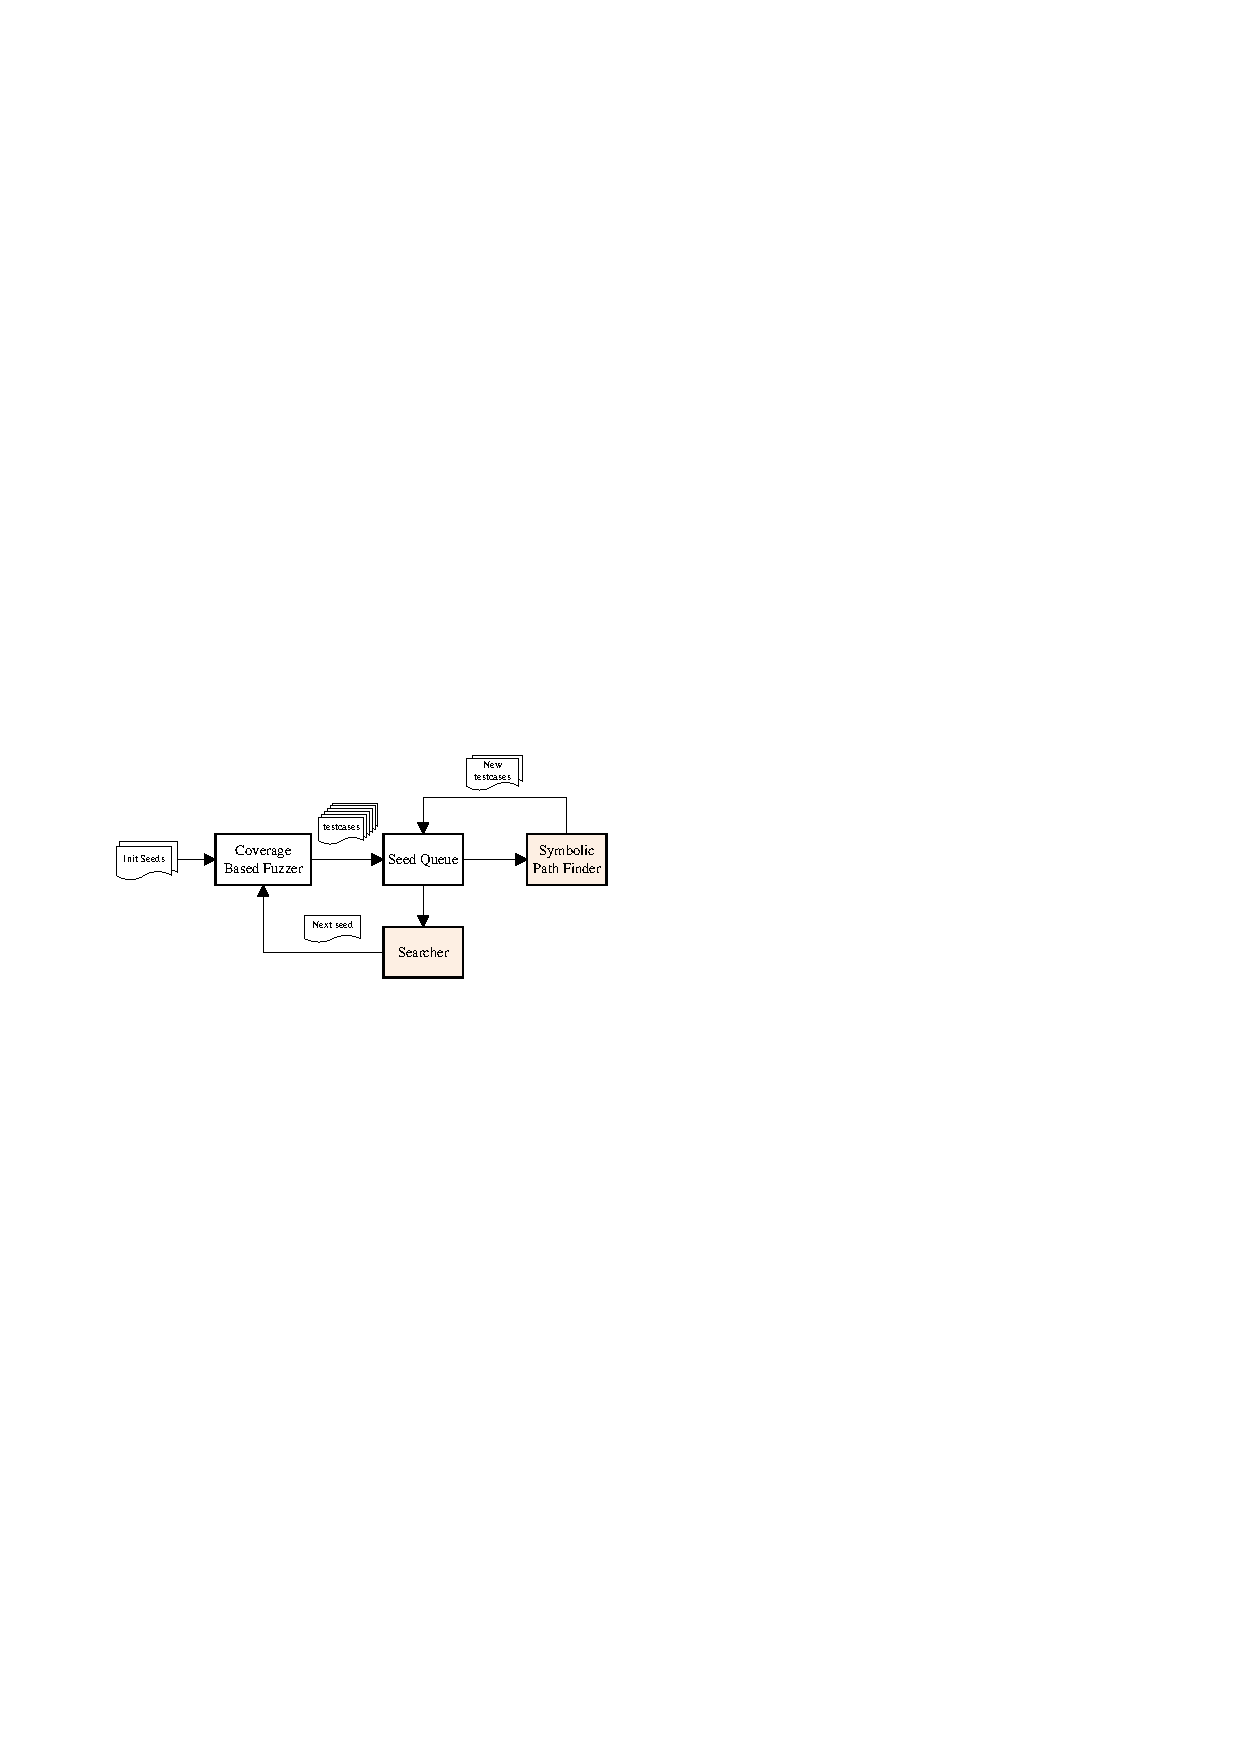
\includegraphics[width=0.7\textwidth]{figures/framework.pdf} 
\caption{High Level Framework.}\label{Framework}
\end{center}
\end{figure}


In summary, this paper makes the following contributions.
\begin{itemize}
\item We introduce a technique to avoid forking more states by postponing the concretization of symbolic pointer to the moment when branch condition depends on such pointer.  
 We also present an optimization namely \emph{symbolic loop bucket} to ease the \textit{path explosion} problem by limiting the looping times to a serial of fixed buckets.

\item A \emph{distance based seed selection} method is proposed to select the most promising seed 
 in the queue according to the runtime information (i.e., path coverage and memory coverage) to improve path discovery when testing time is limited. 

\item We have implemented a prototype based on our method, 
 and the evaluation results on several benchmarks demonstrate the capability of our method for different viewpoints.
\end{itemize}

{\color{blue}{the above is duplication, should be removed.}}

The rest of this paper is organized as follows. 
 The next section describes the basic conception of symbolic execution and hybrid testing. 
 {\color{blue}{give the reference, do not say the next section.}}
 Section~\ref{sec:ease PE} presents the technique details of how we deal with \textit{path explosion} raised from symbolic pointers and loops. The distance based seed selection method is discussed in Section~\ref{sec:seed selection}. Section~\ref{sec:evaluate} describes the implementation of our prototype and the evaluation results. Section~\ref{sec:discussion} discusses the limitations of our work and possible counter measures. Section~\ref{sec:related} reviews the related work, and Section~\ref{sec:conclusion} concludes this paper.
